\documentclass[12pt]{article}
\title{%
The Effects of Phenotypic Plasticity on the Fixation Probability of Mutant Cancer Stem Cells}
\author{Brydon Eastman}
\usepackage[margin=3cm]{geometry}
\usepackage{amsmath,amsfonts,amsthm,amssymb,graphicx,float}

\graphicspath{{../images/}}

\usepackage[title]{appendix}

\usepackage{microtype, url}
\renewcommand{\d}{{\rm d}}
\begin{document}
\maketitle
\begin{abstract}
The cancer stem cell hypothesis claims that tumor growth and progression are driven by a (typically) small niche of the total cancer cell population called cancer stem cells (CSCs). These CSCs can go through symmetric or asymmetric divisions to differentiate into specialised, progenitor cells or reproduce new CSCs. While it was once held that this differentiation pathway was unidirectional, recent research has demonstrated that differentiated cells are more plastic than initially considered. In particular, differentiated cells can de-differentiate and recover their stem-like capacity. Two recent papers have considered how this rate of plasticity affects the evolutionary dynamic of an invasive, malignant population of stem cells and differentiated cells into existing tissue \cite{mohammad, wodarz}. These papers arrive at seemingly opposing conclusions, one claiming that increased plasticity results in increased invasive potential, and the other that increased plasticity decreases invasive potential. Here, we show that what is most important, when determining the effect on invasive potential, is how one distributes this increased plasticity between the compartments of resident and mutant-type cells. We also demonstrate how these results vary, producing non-monotone fixation probability curves, as inter-compartmental plasticity changes. We conclude by demonstrating the stability of these qualitative results over various parameter ranges.

\end{abstract}
\section{Introduction}
%\marginpar{Before I really nit-pick over figure placement, i want to ensure body text is ``okay". Right now there may be jumps in text on the page as each figure is strictly placed}
Cancer invasion is a complex process of the cellular ecosystem and micro-environment. Typically, cancerous cells achieve evolutionary success by mimicking, and subverting, the behaviour of regular, healthy tissues in the host \cite{moh1}. In healthy tissue a distinct stratification of tissue structure is observed where the self-renewal capabilities of terminally differentiated cells rely upon a discrete subclass of the cellular population deemed stem cells \cite{weis2000}. In particular, these stem cells can behave invasively through the process of division and specialisation \cite{moh2}. As healthy, specialised (or differentiated) cells die, the stem cells divide producing the required differentiated cell as a byproduct of mitosis. In this way the population of specialised, terminally differentiated cells is maintained \cite{moh2, watt2000}. However, in order to maintain tissue homeostasis, this mechanism must be controlled by both positive and negative feedback loops. To that effect there is mounting evidence that differentiated cells can de-differentiate back into adult stem cells \cite{watt2000}.

This process of cellular invasion in the tissue driven by a particular niche of cells is very similar to the dynamics observed in invasive cancers. This has led to the cancer stem cell hypothesis that posits that the invasion, metastasis, and regulation of solid tumors are driven by a (typically) small sub-population of cells that behave very much like stem cells \cite{moh3, moh4, moh5, moh6}. In particular, this same behaviour of differentiated cells undergoing some process of de-differentiation and recovering some stem-like properties has been implicated in many forms of cancers experimentally \cite{moh23, moh24, moh25, moh26}.

Recently two papers have mathematically modeled the effect of this stem-cell plasticity and de-differentiation on the evolutionary dynamics of cancer stem cells \cite{mohammad,wodarz}. Both papers are concerned with how the invasive efficacy of mutated stem cells depends upon the degree of de-differentiation considered. In particular, both investigate a situation where a resident type of stem cells and differentiated cells have fully saturated within a population and by introducing a single mutant type within the population the fixation probability of these mutants is recovered. In \cite{mohammad} the authors conclude that as the rate of plasticity increases in a population of cancer stem cells, the fixation probability of mutant stem cells increases. In \cite{wodarz}, however, the author concludes that as the plasticity increases in a population of cancer stem cells, the fixation probability of mutant stem cells decreases. These results are evidently at odds with one another and it is the purpose of this report to reconcile and explain the differing dynamical predictions of these models.

\section{Modeling}

The structure of the models is the same in both papers \cite{mohammad, wodarz}. The authors consider a population of resident stem cells in an equilibrium state. They then introduce a mutant, cancerous stem cell into the wild-type population and investigate the probability that the single mutant achieves fixation as a function of the plasticity of the mutant stem cell. That is, the probability $\rho_S$ that as time $t$ tends to infinity the wild type stem cells have all either died or differentiated and the mutant type stem cells remain for a given de-differentiation rate $\eta$.

\subsection{A Discrete Moran Model}
%\marginpar{Am I going in too much detail for these subsections?}
In \cite{mohammad} the authors consider modeling the birth-death process by way of a Moran model. In particular, the authors consider two types of cells, stem cells ($S_i$) and differentiated cells ($D_i$) where $i\in\{1,2\}$ denotes whether the cells in question are wild-type ($i=1$) or mutant-type ($i=2$). Cells can react and transition between compartments according the following rules (summarised in Figure \ref{MohFig1}). Stem cells undergo division at a rate $r_i$. There is a probability $u_i$ that the stem cell produces both a stem cell $S_i$ and a differentiated cell $D_i$ during division. Similarly, with probability $(1-u_i)$, the stem cell produces two stem cells as the result of this division. Moreover, differentiated cells can reproduce as well at a rate $\tilde{r}_i$. There is a probability $\eta_i$ that this division is asymmetric, producing one stem cell $S_i$ and one differentiated cell $D_i$, and a probability ($1-\eta_i$), that the division is symmetric, producing two differentiated cells $D_i$. Similarly, with probability $d_i$ and $\tilde{d}_i$, the stem cells and differentiate cells die.

\begin{figure}[H]
\begin{center}
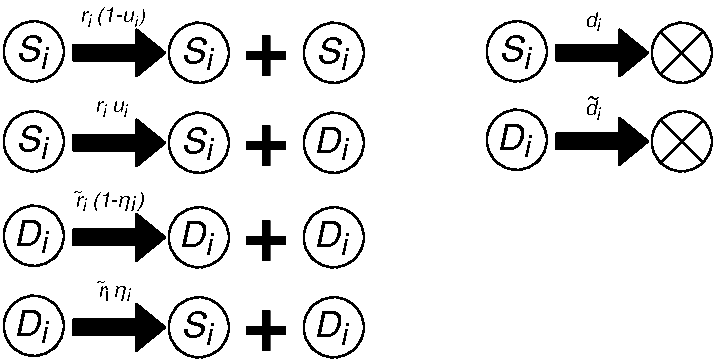
\includegraphics[width=0.7\textwidth]{Moh_Rxns.pdf}
\end{center}
\caption{The differentiation, de-differenation, and death events corresponding to a four-compartment model where $S_i$ and $D_i$ are the stem-cells and differentiated cells for the wild-type ($i=1$) and mutant-type ($i=2$) respectively. Differentiation and de-differentiation events connect the selection dynamics between the two niches.}\label{MohFig1}
\end{figure}

Note that in each of these events the population of stem cells and differentiated cells changes by at most 1 in either direction. Moreover, as births and deaths of cells are assumed to occur instantaneously, the state of the system at any point in time is determined entirely by the state at the previous time. Hence, the particular stochastic process being considered is Markovian. Further, the authors assume that each individual compartment has constant population size across wild and mutant types: i.e. the number of stem cells and the number of differentiated cells remain static, merely what proportion of these stem or differentiated cells are wild or mutant type is the variable.

Let $N_S$ denote the size of the stem cell compartment, $N_D$ the size of the differentiated compartment, and $N=N_S+N_D$ the total number of cells considered. Further, we are concerned primarily with invasion of mutant types; that is, when the number of $S_2$ or $D_2$ cells is at a maximum (equal to $N_S$ or $N_D$). Hence we let $n_S$ and $n_D$ represent the number of $S_2$ or $D_2$ cells. Therefore, the number of $S_1$ or $D_1$ cells is given by $N_S-n_S$ and $N_D-n_D$, respectively. Let $W_S^+(n_S,n_D), W_S^-(n_S,n_D), W_D^+(n_S,n_D)$, and $W_D^-(n_S,n_D)$ represent the transition probabilities corresponding to an increase or decrease by one (represented by the $+$ or $-$ in the superscript) in the number of stem cells or differentiated cells (represented by the $S$ or the $D$ in the subscript). Then, if $1/N$ is the duration of each time step in this model, one can represent the following master equation for the probability density function of the stochastic process as follows \cite{mohammad}:
%\marginpar{Should I remove the formulae in (1)-(5)? and (6)}
\begin{align}
\frac{1}{N}\frac{\partial p(n_S,n_D;t)}{\partial t}&=W_S^+(n_S-1,n_D)\, p(n_S-1,n_D;t) + W_S^-(n_S+1,n_D)\, p(n_S+1,n_D;t)\nonumber\\
&\quad
+ W_D^+(n_S,n_D-1)\, p(n_S,n_D-1;t) + W_D^-(n_S,n_D+1)\, p(n_S,n_D+1;t)\nonumber\\
&\quad
-(W_S^+(n_S,n_D)+W_D^+(n_S,n_D)+W_S^-(n_S,n_D) \nonumber\\
&\quad
+W_D^-(n_S,n_D))\, p(n_S,n_D;t)  \, ,
\label{MohRef1}
\end{align}
where the transition probabilities are given as follows:
\begin{align}
W_S^+(n_S,n_D) &= \left(r_2\,(1-u_2)\,n_S+\tilde{r}_2\,\eta_2\,n_D\right)\left(\frac{N_S-n_S}{N_S}\right)\label{MohRef2}\\
W_S^-(n_S,n_D) &= \left(r_1\,(1-u_1)\,(N_S-n_S)+\tilde{r}_1\,\eta_1\,(N_D-n_D)\right)\left(\frac{n_S}{N_S}\right)\\
W_D^+(n_S,n_D) &= \left(\tilde{r}_2\,(1-\eta_2)\,n_D+r_2\,u_2\,n_S\right)\left(\frac{N_D-n_D}{N_D}\right)\\
W_D^-(n_S,n_D) &= \left(\tilde{r}_1\,(1-\eta_1)\,(N_D-n_D)+r_1\,u_1\,(N_S-n_S)\right)\left(\frac{n_D}{N_D}\right).
\label{MohRef3}
\end{align}
% With equations (\ref{MohRef1}) and (\ref{MohRef2}-\ref{MohRef3}) are reproduced from \cite{mohammad}.

The results of Figure \ref{combine_fig}--a clearly demonstrate that fixation probability increases as plasticity of the mutant increases. In particular, when the resident wild type cells were given no plasticity and the mutant type cells plasticity was treated as a variable it was observed that increasing the mutant types plasticity gave these mutant types a greater invasive potential when placed in a population dominated by wild types population.

\subsection{A Continuous Gillespie Model}
\begin{figure}
\[\begin{array}{cc}
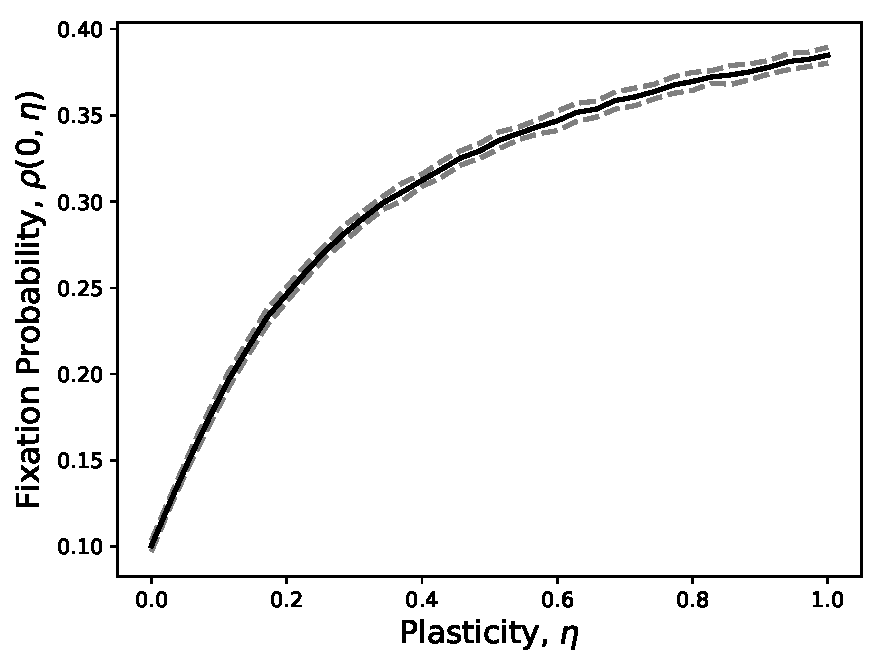
\includegraphics[width=0.37\textwidth]{moh_combine.pdf}&
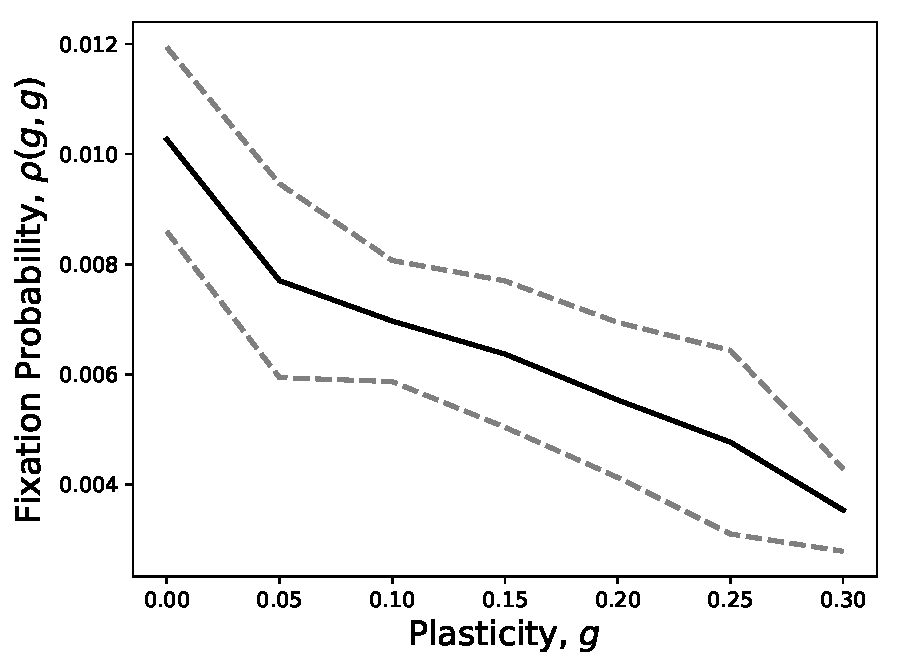
\includegraphics[width=0.37\textwidth]{wod_combine.pdf}\\
\text{a) The Discrete Moran Model} & \text{b) The Continuous Gillespie Model}
\end{array}\]
\caption{This Figure shows the results of a simulation of both the discrete Moran model from \cite{mohammad} and the continuous Gillespie model from \cite{wodarz} where the wild-type differentiated cells are completely non-plastic. The figures show the contrasting results where in (a) the fixation probability increases as mutant-type plasticity increases and in (b) the fixation probability decreases as mutant-type plasticity increases.}\label{combine_fig}
\end{figure}
%\marginpar{Figure a holdover until my code finishes running}

On the other hand, in \cite{wodarz} the author aims to describe the dynamics of stem cell invasion not merely by considering births and deaths and the selective pressures therein, but by directly considering the positive and negative feedbacks that control differentiation and de-differentiation in the stem cell hierarchy. To this end, the author constructs multiple systems of differential equations that model the behaviour of stem cells and differentiated cells under various assumptions. The key differences between this paper and \cite{mohammad}, are in the details of these models. In particular, the author does not limit themselves to constant population size of stem cell and differentiated cell compartments. As before, the author considers a four compartment model where $S_i$ represents the stem cells and $D_i$ represents the differentiated cells: 

\begin{equation}
\begin{array}{rl}
\frac{\d S_i}{\d t}&= \hat{r}_i\,S_i\,(2\,p_i-1)+g_i\,D_i\vspace*{5pt}\\
\frac{\d D_i}{\d t}&= 2\,\hat{r}_i\,S_i\,(1-p_i)-\alpha_i\,D_i-g_i\,D_i
\end{array}\label{wodDE}
\end{equation}
where $i\in\{1,2\}$ represents the wild type ($i=1$) and mutant type ($i=2$), as before.

While the author of \cite{wodarz} does not frame the model as a reaction network, it is not hard to recover the set of reactions from the differential equations. These are presented in Figure \ref{wodarzRxns}. 

\begin{figure}
\begin{center}
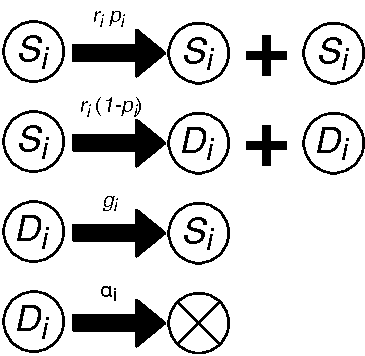
\includegraphics[width=0.35\textwidth]{Wodarz_Rxns.pdf}
\end{center}
\caption{Figure demonstrating the suite of reactions captured by the Wodarz Model. Stem cell division is always assumed to be symmetric, producing either two new stem cells or two progenitor cells.}\label{wodarzRxns}
\end{figure}

One should note that if $p_i\neq \frac{\alpha_i-g_i}{2\,\alpha_i}$, then the only equilibrium is $S_i=D_i=0$. Otherwise, the entire set $[S_i,D_i]=[S_i,(r_i/\alpha_i)\,S_i]$ is an equilibrium.  These results do not coincide with what is observed in experiments. The author argues that feedback on the division rate, self-renewal probability, and de-differentiate rate occurs in order to maintain finite-size cell populations. To model this, it is assumed that $\hat{r}_i$, $p_i$, and $g_i$ are decreasing functions of the cell population sizes in the following way:
\[
\hat{r}_i=\frac{\hat{r}_i'}{1+h_{i,1}\,D_i^{k_{i,1}}}, \quad p_i=\frac{p_i'}{1+h_{i,2}\,D_i^{k_{i,2}}}, \quad g_i=\frac{g_i'}{1+h_{i,3}\,S_i^{k_{i,3}}}
\]
In this case, the model permits an equilibrium point internal to the first quadrant that is stable when $p_i>\frac{\alpha_i-g_i}{2\,\alpha_i}$.

To numerically establish the fixation probability the following experiments were run. The author begun by placing $S_1$ and $D_1$ at the equilibrium values and then introduced a single mutant stem cell, $S_2=1$ and $D_2=0$. Gillespie simulations were then performed \cite{gillespie} for many realisations (more than $10^8$). The fraction of simulations in which the mutants fixated was recorded and from this the fixation probability was estimated. This was done for various values of de-differentiation rates $g=g_1=g_2$.

In contrast to the results of the discrete Moran model in Figure \ref{combine_fig}--a, Figure \ref{combine_fig}--b shows that the fixation probability of a neutral mutant decreases when the de-differentiation rate increases in the continuous Gillespie model.

\section{Reconciliation of Previous Results}\label{recon}

In the Wodarz model there are four parameters considered for each cell-type (mutant or wild) ($p_i, \hat{r}_i, \alpha_i, g_i$) while in the Shirayeh model there are six ($r_i,\tilde{r}_i, d_i, \tilde{d}_i, \eta_i, u_i$). The biggest difference between these parameters is that in \cite{wodarz} the numbers $p_i$ and $r_i$ are both functions of $D_i$, and $g_i$ is a function of $S_i$.

Moreover, \cite{wodarz} considers four reactions between stem cell and differentiated cell compartments 
\[S_i\to S_i+S_i \,\, , \,\, S_i\to D_i+D_i \,\, , \,\, D_i\to S_i \,\, , \,\, D_i\to \emptyset.\] 
Whereas in \cite{mohammad} there are six
\[
S_i\to S_i+S_i \,\, , \,\, S_i\to S_i+D_i \,\, , \,\, D_i\to D_i+D_i \,\, , \,\, D_i\to D_i+S_i \,\, , \,\, S_i\to\emptyset \,\, , \,\, D_i\to\emptyset.
\]

However, all the reactions from \cite{mohammad} can be recovered in the Wodarz model \cite{wodarz}. In particular, in order for stem cells to die they must first differentiate and then the differentiated cells must both die. In order to obtain asymmetric stem cell division, the stem cells must first divide into two differentiated cells, then one of the differentiated cell must de-differentiate back into a stem cell. Suppose a differentiated cell first differentiates into a stem cell and then the resultant stem cell symmetrically differentiates. Therefore, the differentiated cell has symmetrically divided. Further, suppose one of those resultant differentiated cells de-differentiates back into a stem cell, then the differentiated cell has asymmetrically divided. In this way all the reaction dynamics of the model from \cite{mohammad} have been recovered by multiple reactions from the model by \cite{wodarz}.

This realisation lends credence to the theory that the models should, hopefully, predict similar qualitative dynamics. To that end, we begin by creating differential equations via the reactions given in Figure \ref{MohFig1} and compare them to the differential equations presented in \cite{wodarz}. By making the mass-action assumption, it is easy to derive
\begin{equation}
\begin{array}{rl}
\frac{\d S_i}{\d t}&=\tilde{r}_i\,\eta_i\,D_i+r_i\,(1-u_i)\,S_i-d_i\,S_i\vspace*{5pt}\\
\frac{\d D_i}{\d t}&=\tilde{r}_i\,(1-\eta_i)\,D_i+r_i\,u_i\,S_i-\tilde{d}_i\,D_i.
\end{array}\label{mohDE}
\end{equation}
Contrasting (\ref{mohDE}) with (\ref{wodDE}) it is not hard to derive the following relations. To frame the Wodarz model \cite{wodarz} in terms of parameters from \cite{mohammad},
\begin{align*}
p_i&=1-\frac{r_i\,u_i}{2\,(r_i-d_i)}\\
\hat{r}_i&=r_i-d_i\\
\alpha_i&=\tilde{d}_i-\tilde{r}_i\\
g_i&=\tilde{r}_i\,\eta_i
\end{align*}
conversely, framing the model in \cite{mohammad} in terms of parameters from the Wodarz model \cite{wodarz} we leave $d_i$ and $\tilde{d}_i$ as free parameters, then
\begin{align*}
r_i&=d_i+\hat{r}_i\\
\tilde{r}_i&=\tilde{d}_i-\alpha_i\\
\eta_i&=\frac{g_i}{\tilde{d}_i-\alpha_i}\\
u_i&=2\frac{\hat{r}_i\,(1-p_i)}{d_i+\hat{r}_i}.
\end{align*}

Hence the qualitative dynamics of (\ref{mohDE}) are dynamically equivalent to those of (\ref{wodDE}), under a renaming of parameters. Moreover, these formulae allow us to more carefully compare the two systems predictions under differing notations and parameter choices, as the formulae provide a way to transcribe parameter values and notational choices from one system into the notation of the other. In particular, note that the two plasticity parameters $g_i$ and $\eta_i$ can be compared directly, as they are just linear, increasing functions of one another. Hence an increase in $g_i$ is analogous to an increase in $\eta_i$ (and vice versa). Moreover, $\eta_i=0$ is analogous to $g_i=0$.

Negative feedback on production rates is modeled in the model put forth by \cite{mohammad}, but not as explicitly as in \cite{wodarz}. In particular, the last factor in the transition probabilities of \cite{mohammad} provide this bias. If $n_S$ is high, or the number of stem cells is close to maximum, then the transition probability $W_S^+$ is near zero, due to the $(N_S-n_S)/N_S$ factor at the end. Hence when the number of mutant stem cells is high, the probability of making more mutant stem cells is lowered (this mimics the behaviour observed in the $g_2(S_2)$ function in the Wodarz model \cite{wodarz}). Similarly the $n_S/N_S$ term in the $W_S^-$ transition probability creates pressure where creating more wild-type stem cells is less likely in the presence of many wild-type stem cells (similar to the $g_1(S_1)$ function in the Wodarz model \cite{wodarz}). Analogous behaviour occurs in the $W_D^{\pm}$ probabilities, mimicking the behaviour of the $\hat{r}_i$ and $p_i$ functions decreasing as $D_i$ increases. 

In the finite population size model, negative feedback on (de--)differentiation rates and production rates are governed by the select pressures inherit in finite population sizes, whereas in the unbounded population size model these same feedback mechanisms are modeled by non-constant, non-linear reaction rates. 

A more subtle difference between the two systems is due, in part, to a lack of clarity in notational differences. In the original presentation of \cite{wodarz} the $i$ subscripts were not present (though different values of the same parameter between compartments was implied in the figure descriptions). Among other things, this obscures the fact that $g$ (the parameter representing de-differentiation, or plasticity) is being altered at the same rate for both the mutant-type population and for the resident-type population. Hence, the plots in Figure \ref{combine_fig}--b really plot the fixation probability $\rho(g_1,g_2)$ along the diagonal cross-section of the first quadrant, that is the plots show
\[
\frac{\partial}{\partial g}\left(\rho(g_1,g_2)\big|_{g_1=g_2=g}\right)<0
\]
whereas the plots in Figure \ref{combine_fig}--a show
\[
\frac{\partial}{\partial \eta_2}\left(\rho(\eta_1,\eta_2)\big|_{\eta_1=0}\right)>0.
\]
The tacit assumption in \cite{mohammad} is that part of the phenotypic difference between the mutant stem cells and the resident stem cells is that resident stem cells have no plasticity and mutant stem cells do have plasticity. The analysis then focuses around qualifying the effects of this plasticity. Contrast this, the tacit assumption in \cite{wodarz} is that the mutant and resident stem cells are phenotypically different in some other way and share the same plasticity rate.

To conclude, we wished to consider measuring $\rho(\eta, \eta)$ for $0\le\eta\le 1$ in the discrete Moran model (that is, the fixation probability from \cite{wodarz} in the model by \cite{mohammad}) and to measure $\rho(0, g)$ for $0\le g\le 1$ in the continuous Gillespie model (that is, the fixation probability from \cite{mohammad} in the model by \cite{wodarz}). In particular, as can be seen in Figure \ref{moh_wod_switch}, we have recovered the results of the contrasting models. That is, in Figure \ref{moh_wod_switch}--a we see that $\rho(\eta, \eta)$ is a decreasing function of $\eta$ as was seen in \cite{wodarz} (Figure \ref{combine_fig}--b) and that $\rho(0,g)$ is an increasing function of $g$ as was seen in \cite{mohammad} (Figure \ref{combine_fig}--a).


\begin{figure}[H]
\[
\begin{array}{cc}
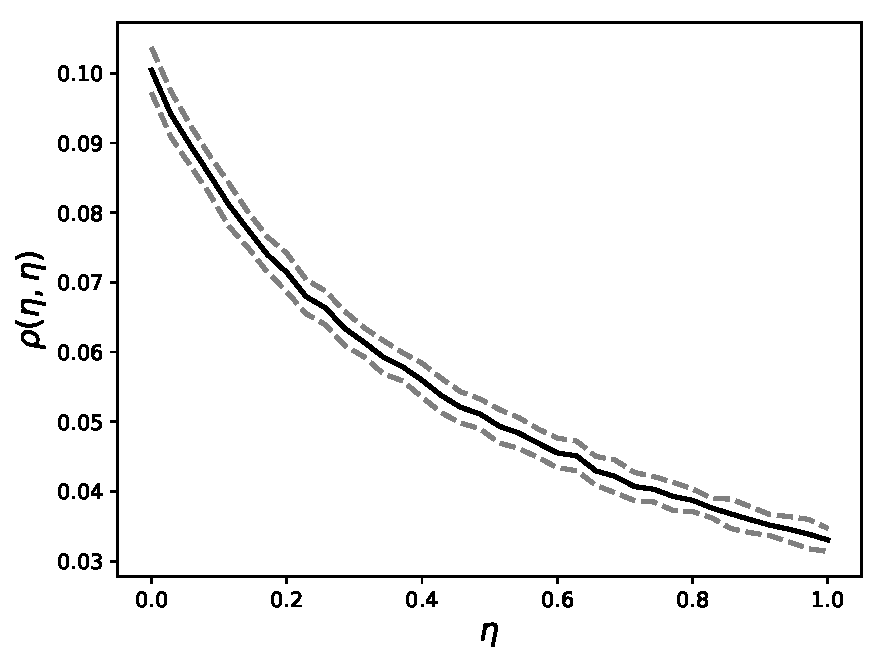
\includegraphics[width=0.37\textwidth]{moh_in_wod.pdf}&
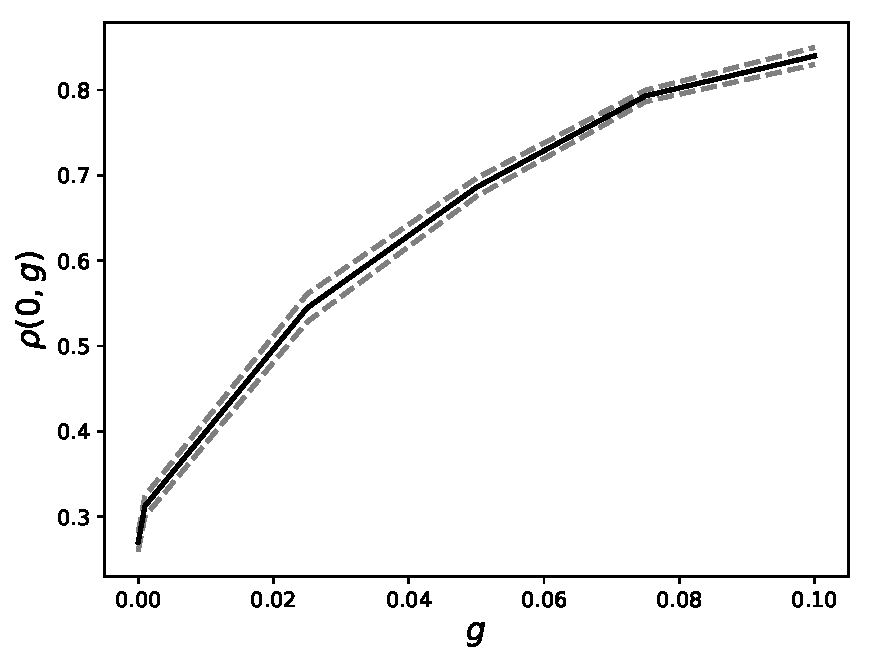
\includegraphics[width=0.37\textwidth]{wod_in_moh.pdf}\\
\text{a) The Discrete Moran Model}&\text{b) The Continuous Gillespie Model}
\end{array}
\]
\caption{The figure indicates that when varying both the wild-type and mutant-type plasticity parameters at the same rate in the discrete Moran models, the fixation probability function is negatively sloped. Similarly, when increasing only the mutant-type plasticity parameter and keeping the wild-type plasticity parameter at zero in the continuous Gillespie model, the fixation probability function increases. Note that these results are similar to what was observed in Figure \ref{combine_fig}, just with the modelling framework switched.}\label{moh_wod_switch}
\end{figure}

\section{Further Results}\label{further}
The results of Section \ref{recon} demonstrate that it is vitally important to consider how a change in plasticity in a mutant type affects a change in plasticity of a wild type, if at all.
In particular, the authors of \cite{mohammad} and \cite{wodarz} were effectively answering different research questions. In \cite{mohammad} the authors were concerned with what the effect of increased plasticity in a mutant-type would have on fixation probability assuming the wild-type stayed the same. This corresponds to a case where the mutant-type gains increased plasticity as part of the mutation. Moreover, this assumes that this increased plasticity in the mutant type does not have any effects on the plasticity in the resident type. Contrarily, in \cite{wodarz} the authors assume that the increased plasticity is common to both the mutant and wild type stem cells. This could be the case where an increased mutant-type plasticity affects the wild-type stem cells by some kind of increased selective pressure, or via a change in the micro-environment thus influencing the wild-type to also become more plastic.

As Section \ref{recon} made it apparent that the Gillespie model and Moran model are effectively equivalent means of modeling this phenomenon, we consider Moran simulations henceforth. This is done purely because Moran simulations are less computationally expensive than Gillespie simulations.

\begin{figure}[ht]
\begin{center}
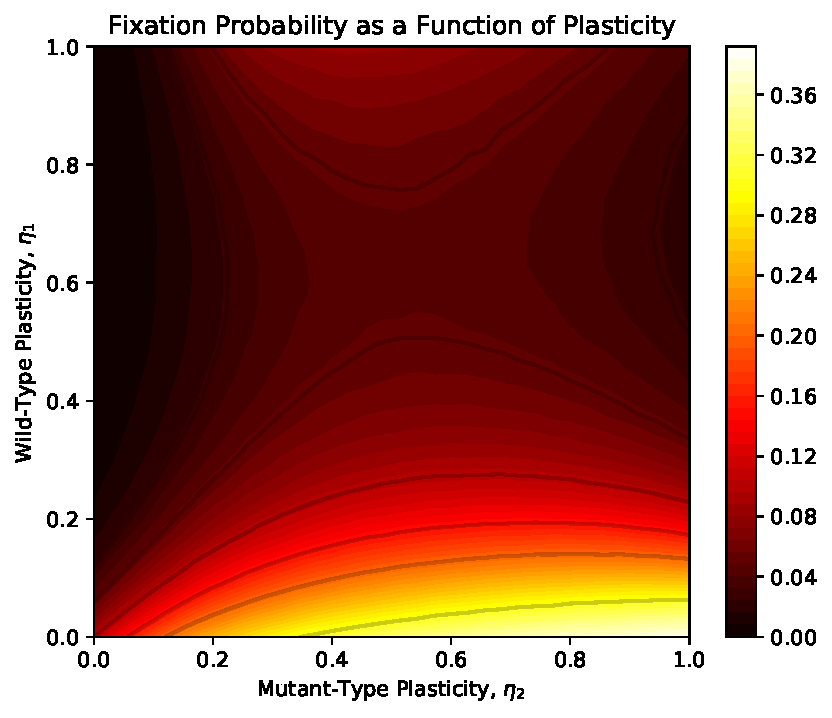
\includegraphics[width=0.74\textwidth]{contourplot.pdf}
\end{center}
\caption{A contourplot demonstrating the fixation probability as a function of both de-differentiation parameters. It indicates that increasing the mutant-type de-differentiation parameter does not always result in increased fixation of mutant-type stem cells, even when keeping the wild-type de-differentiation parameter constant.}\label{contour}
\end{figure}

We consider varying both $\eta_1$ and $\eta_2$ (the plasticity of the wild-type and mutant-type cells) independently of one another. Since $\eta_1$ and $\eta_2$ are probabilities, we varied them over the closed unit square $[0,1]\times[0,1]$ in a $36\times36$ grid. At each point in the grid we calculated the fixation probability of the mutant-type stem cells. Further details of the numerical simulation, and a link to the code, can be found in Appendix \ref{exp}. 

The purpose of the experiment was to further investigate the exact interplay between plasticity in the two compartments on the fixation probability. However, there are 6 other parameters to consider,  $r_i, \tilde{r}_i,$ and $u_i$. In order to investigate the direct effect of a change in plasticity on the fixation probability in isolation, we considered the case where relative fitness was the same in the stem and differentiated cells (that is, $r_i=\tilde{r}_i$).

We further considered experiments where the relative fitness of the mutant-type cells ($r_2=\tilde{r}_2$) were varied along with the de-differentiation probabilities ($\eta_1$ and $\eta_2$). Moreover, to further analyse the stability, we considered varying the differentiation probability ($u_2$) of the mutant-type cells along with the de-differentiation probabilities.

In the case of the neutral mutant (where $r_2=\tilde{r}_2=r_1=\tilde{r}_1$ and $u_2=u_1$), the results are summarised in Figures \ref{contour}, \ref{constantEta1Stack}, and \ref{avg_eta1_plot}. The contour plot in Figure \ref{contour} indicates the fixation probability as a function of both de-differentiation parameters. It indicates that in general, increasing $\eta_2$, the de-differentiation probability of the mutant cells, increases the fixation probability. Moreover, this fixation probability is maximal for $(\eta_1, \eta_2) = (0, 1)$. However, it also shows that for large enough $\eta_1$, increasing $\eta_2$ will not always result in an increased fixation probability. In the extreme case, where $\eta_1=1$, increasing $\eta_2$ initially increases the fixation probability, but eventually this fixation probability decreases as $\eta_2$ is closer to $1$.

This result can be seen more clearly in Figure \ref{constantEta1Stack}, where the fixation probability is plotted for constant values of $\eta_1$ as a function of varying $\eta_2$. When $\eta_1=0$ the fixation probability is a concave down, increasing, saturating function of $\eta_2$. However, for $\eta_1=0.2$ the fixation probability is no longer strictly increasing and undergoes a change in concavity early on. As $\eta_1$ is increased further the fixation probability is no longer a strictly increasing function of $\eta_2$ but initially increases and eventually decreases as $\eta_2$ becomes larger. For larger $\eta_1$ the fixation probability function decreases over a larger range of $\eta_2$ and decreases more drastically. Conversely, as $\eta_1$ is increased, the average fixation probability of the mutant-type cells is increased. That is, for $\eta_1=0.8$, the maximum of $\rho(0.6, \eta_2)$ is around $0.045$ (or 4.5\%), but the maximum of $\rho(1, \eta_2)$ is closer to $0.075$ (or 7.5\%). This can be recovered by recognising the saddle-like behaviour of Figure \ref{contour}. This symmetry can be explained similarly, as $\eta_1$ increases, more wild-type differentiated cells are de-differentiating into stem-cells. This removes selective pressure from mutant-type differentiated cells, allowing these mutant-type cells to grow larger and, for appropriate values of $\eta_2$, de-differentiate back into mutant-type stem cells.

\begin{figure}[ht]
\begin{center}
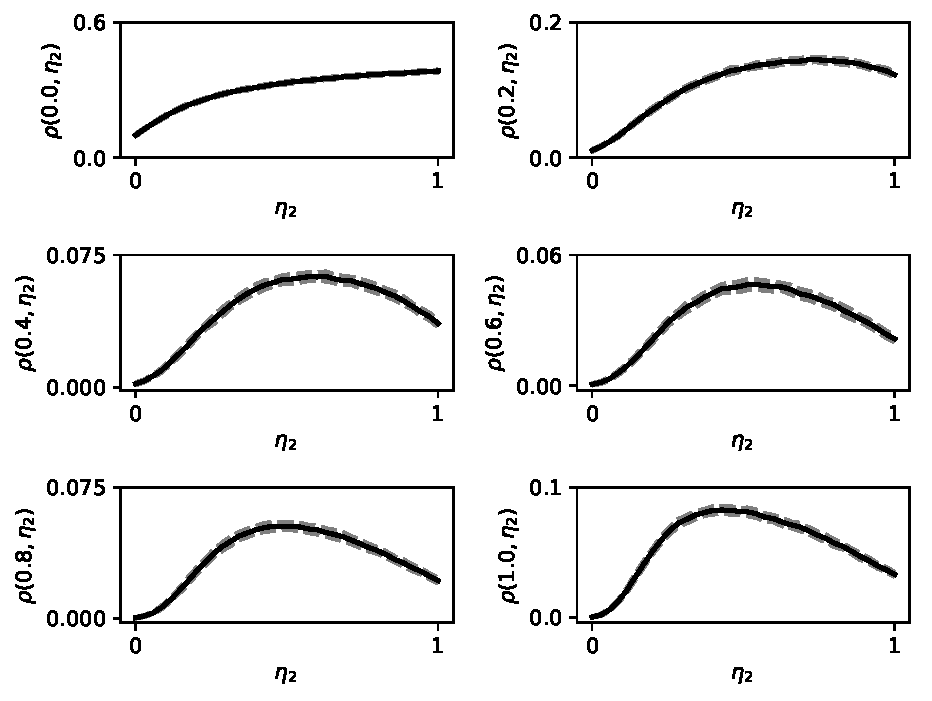
\includegraphics[width=0.74\textwidth]{constant_eta1_stackplot.pdf}
\end{center}
\caption{A stackplot demonstrating the fixation probability as a function of the de-differentiation probability $\eta_2$ for various choices of $\eta_1$. The solid line is the calculated fixation probability and the dashed lines indicate one deviation by the standard error of the mean.}\label{constantEta1Stack}
\end{figure}

This non-monotonic fixation probability function is an interesting phenomenon. This implies that for particular parameter sets, it is actually worse for mutant type stem cell fixation to increase the rate at which mutant differentiated cells de-differentiate into mutant stem cells. This is non-obvious, as one would assume increasing the pool of mutant stem cells, by decreasing the pool of mutant differentiated cells, is vital to the fixation of the mutant stem cells. However, by decreasing the pool of mutant differentiated cells, the wild type differentiated cells have a selective pressure removed and can see an increased response in growth. For large enough $\eta_1$, these wild type differentiated cells can de-differentiate back into wild type stem cells and thus provide a selective disadvantage to the mutant stem cells. This is an important phenomenon to fully understand. Much of the results of Section \ref{stab} is to indicate that this phenomenon persists over a wide range of parameter space and is not the result of a particular, lucky set of parameters.

The original paper by \cite{mohammad} considered only a particular constant $\eta_1$ value while allowing $\eta_2$ to vary. Thus far we have considered various constant $\eta_1$ values and noted interesting dynamics occurring. In the paper by \cite{wodarz}, they considered varying $\eta_1$ as a linear function of $\eta_2$ (in their particular case, $\eta_1$ was identically $\eta_2$). In the next set of experiments we considered varying $\eta_1$ as other linear functions of $\eta_2$. 

In the first plot in Figure \ref{eta_stack}, we note that, compared to the $\eta_1=\eta_2$ case, in general the effect is a decrease in fixation probability for $\eta_2$ smaller than, approximately, $0.55$, and an increase in fixation probability as $\eta_2$ reaches its maximum. In this scenario, the initial decrease in fixation probability is intuitive. A more plastic wild-type compartment would allow more wild-type stem cells to be created and hence result in a selective pressure on mutant-type stem cells, resulting in less probable fixation for the mutant cells. However, when $\eta_2$ is sufficiently large, than the difference between $\eta_2$ and $\eta_1$ is less pronounced. This is similar to the theme observed in Figure \ref{constantEta1Stack}. For large enough values of $\eta_2$ the selective pressures from the more plastic wild-type stem cells are reduced. Moreover, in these scenarios the smaller de-differentiation value compartment has a selective advantage in production of differentiated cells, and both differentiated and stem cell compartments are necessary for fixation.

In the second plot in Figure \ref{eta_stack}, we note that in general for $\eta_1$ smaller than $\eta_2$ we, mostly, observe that the fixation probability is increased (compared to the $\eta_1=\eta_2$ case). This is intuitive, when $\eta_1$ is smaller, wild-type stem cells are being produced less quickly than mutant-type stem cells. Hence mutant-type stem cells have a selective advantage for invading. However, when $\eta_2$ is near $1.0$ we observe a very slight dip in fixation probability. In these scenarios, the mutant cells are almost always de-differentiating. Hence the $S_2$ compartment is filling faster while the $D_2$ compartment is draining faster. Even though $\eta_1<\eta_2$, $\eta_1$ is still appreciably non-zero, hence the $D_1$ compartment has a selective advantage due to the small size of the $D_2$ compartment. Therefore, both wild types perform well and fixate with slightly more frequency.

In the third and fourth plots of Figure \ref{eta_stack}, the situation behaves similarly to the first two plots. When $\eta_1>\eta_2$ there is an initial advantage for the wild-type cells that disappears as $\eta_2$ becomes sufficiently large. Contrarily, for $\eta_1<\eta_2$ there is an initial advantage for the mutant-type cells that disappears only when $\eta_2$ becomes sufficiently large. What is unique about these two cases is the loss of monotonicity. In each experiment in the third plot of Figure \ref{eta_stack}, increasing the plasticity parameter $\eta_2$ also increases $\eta_1$, but in this experiment $\eta_1$ initially increases fast enough that the selective disadvantage for wild-type cells imposed by larger $\eta_2$ is offset by the selective advantage for wild-type cells granted by larger $\eta_1$. However, past a certain point the benefit in fixation success for the wild-type cells as a function of $\eta_1$ begins to saturate and become outpaced by the selective advantage imposed by larger $\eta_2$. The fourth plot behaves in a similar fashion to the third plot. For smaller $\eta_1$ initially the fixation probability increases. As $\eta_2$ first begins to increase, $\eta_1$ increases too but at a slower rate. The effect of this initial slow increase in $\eta_1$ is offset by the growing of $\eta_2$, hence the fixation probability function is positively sloped. As $\eta_2$ becomes larger yet, the increase in $\eta_1$ starts to effect the evolutionary dynamics and the fixation probability starts to decrease.

\begin{figure}[H]
\begin{center}
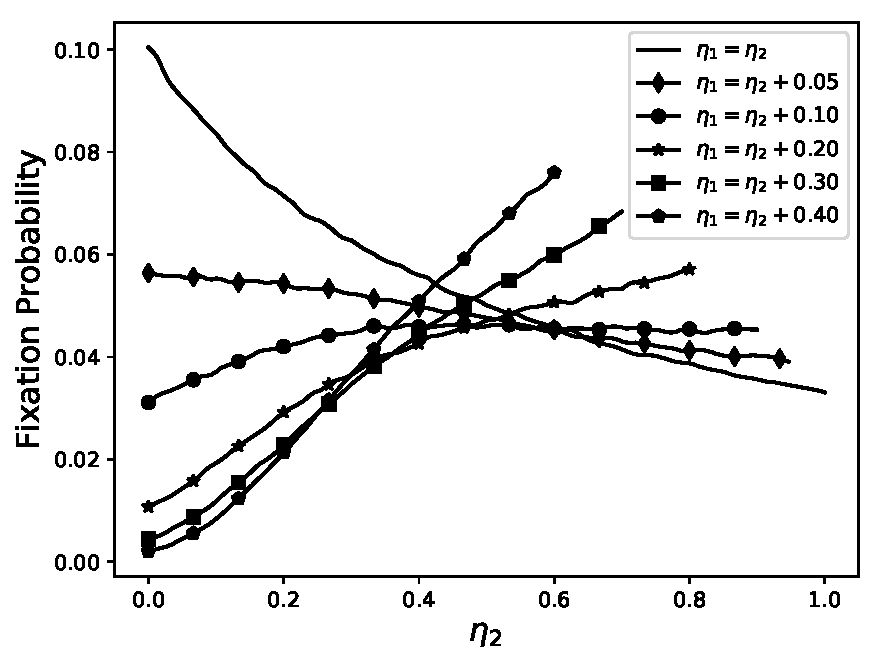
\includegraphics[width=0.46\textwidth]{eta_plus_const.pdf}
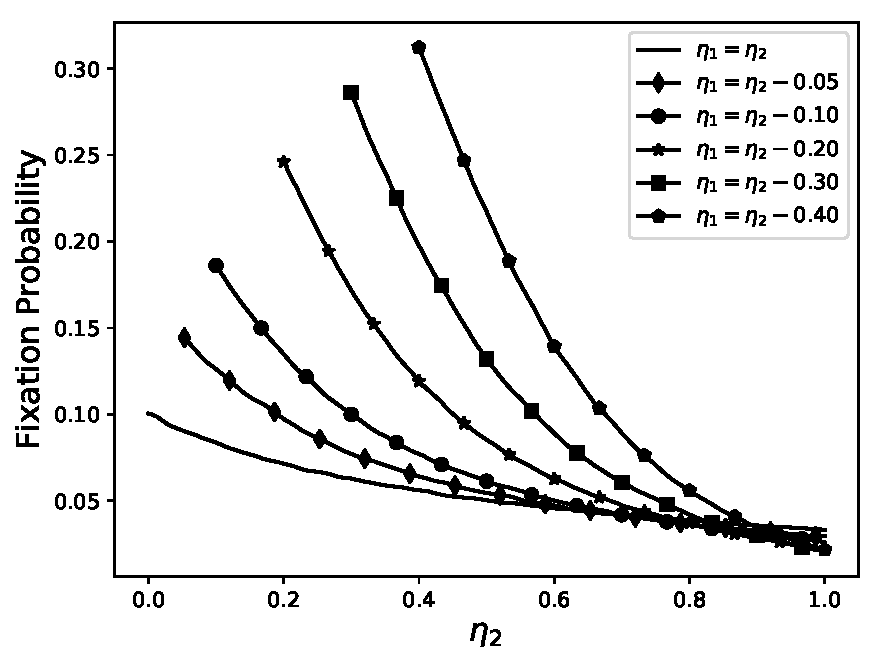
\includegraphics[width=0.46\textwidth]{eta_minus_const.pdf}\\
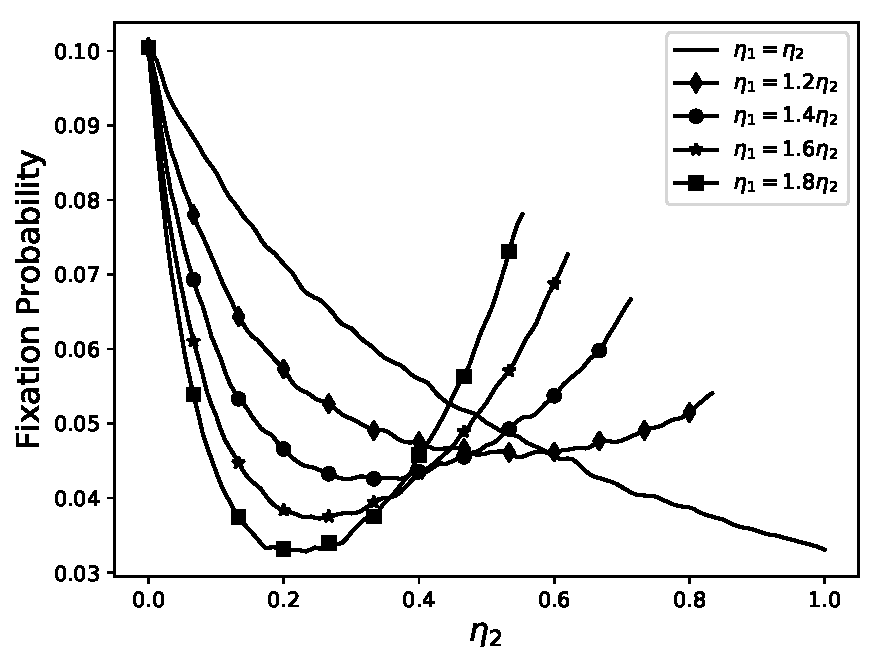
\includegraphics[width=0.46\textwidth]{eta_times_const.pdf}
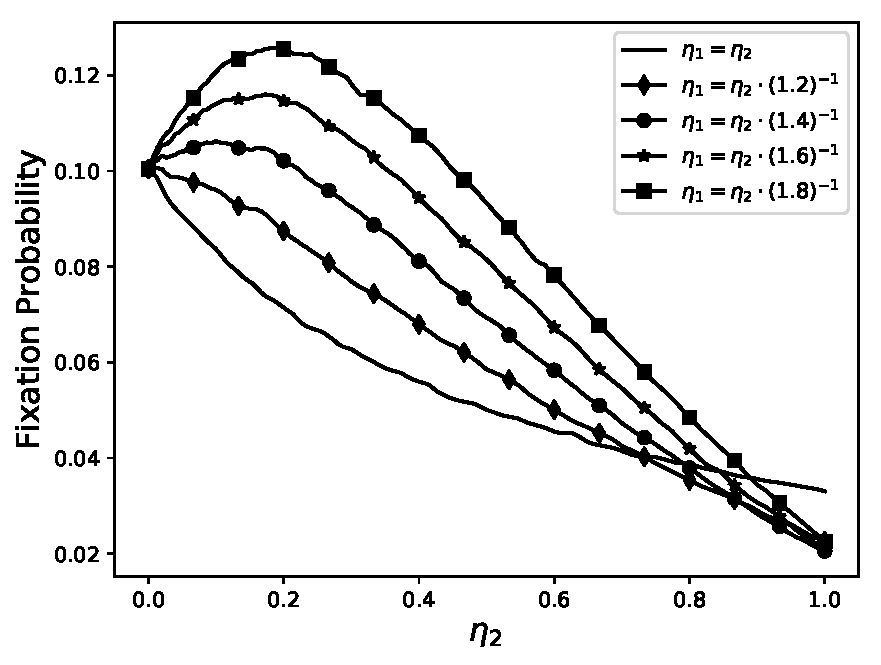
\includegraphics[width=0.46\textwidth]{eta_div_const.pdf}
\end{center}
\caption{The effects on fixation probability by varying $\eta_1$ as a function of $\eta_2$.}\label{eta_stack}
\end{figure}

When examining Figure \ref{contour}, it appears that in general the fixation probability increases. Moreover, when the fixation probability is increasing, it obtains a larger value. That is, for increasing $\eta_1$ the fixation probability is, in general, decreasing. This effect raises the question that in general, in a heterogeneous population of wild-type stem cells where deviations in de-differentiation probability $\eta_1$ can be observed, what might be the expected effect on the fixation probability. To that end, we modeled the average fixation probability as a function of $\eta_2$ averaged over all values of $\eta_1$. That is,

\[\langle\rho(\eta_2)\rangle = \int_0^1 \rho(\eta_1, \eta_2)\,f(\eta_1)\,\d \eta_1\]
where $f(\eta_1)$ is the probability density function for $\eta_1$ in this case taken to be uniform. The result, as presented in Figure \ref{avg_eta1_plot}, is a non-monotone function of $\eta_2$ with a unique maximum, suggesting that in general, increasing the plasticity rate of the mutant-type stem cell will not always result in increased fixation probability, but may be harmful to the mutant-type cells.

\begin{figure}[H]
\begin{center}
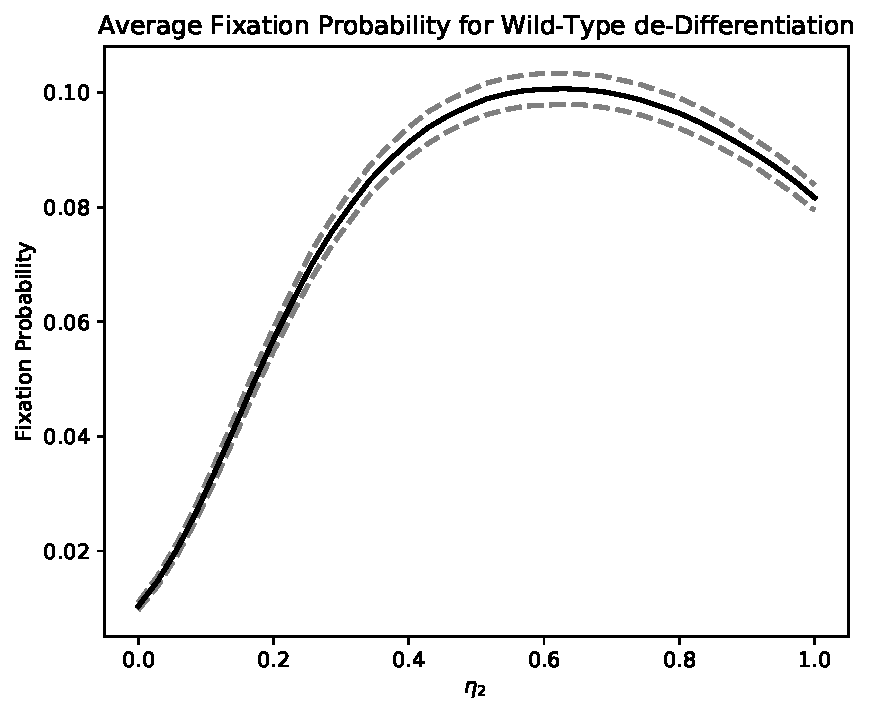
\includegraphics[width=0.74\textwidth]{avg_eta1_plot.pdf}
\end{center}
\caption{The mean fixation probability as a function of $\eta_2$ with the mean taken over the parameter $\eta_1$ assuming a uniform distribution. The dashed bars indicate a single deviation by standard error of the mean.}\label{avg_eta1_plot}
\end{figure}

\subsection{Stability Analysis}\label{stab}

The previous results were all obtained for the neutral mutant. To demonstrate the generality of these results and their independence on particular parameter choices, we repeated the analysis for varying parameters. In particular, we varied the relative fitness of the mutant-types, $r_2=\tilde{r}_2$, and the probability of differentiation of the mutant types, $u_2$. The technical details can be found in Appendix \ref{exp}.


\begin{figure}[H]
\begin{center}
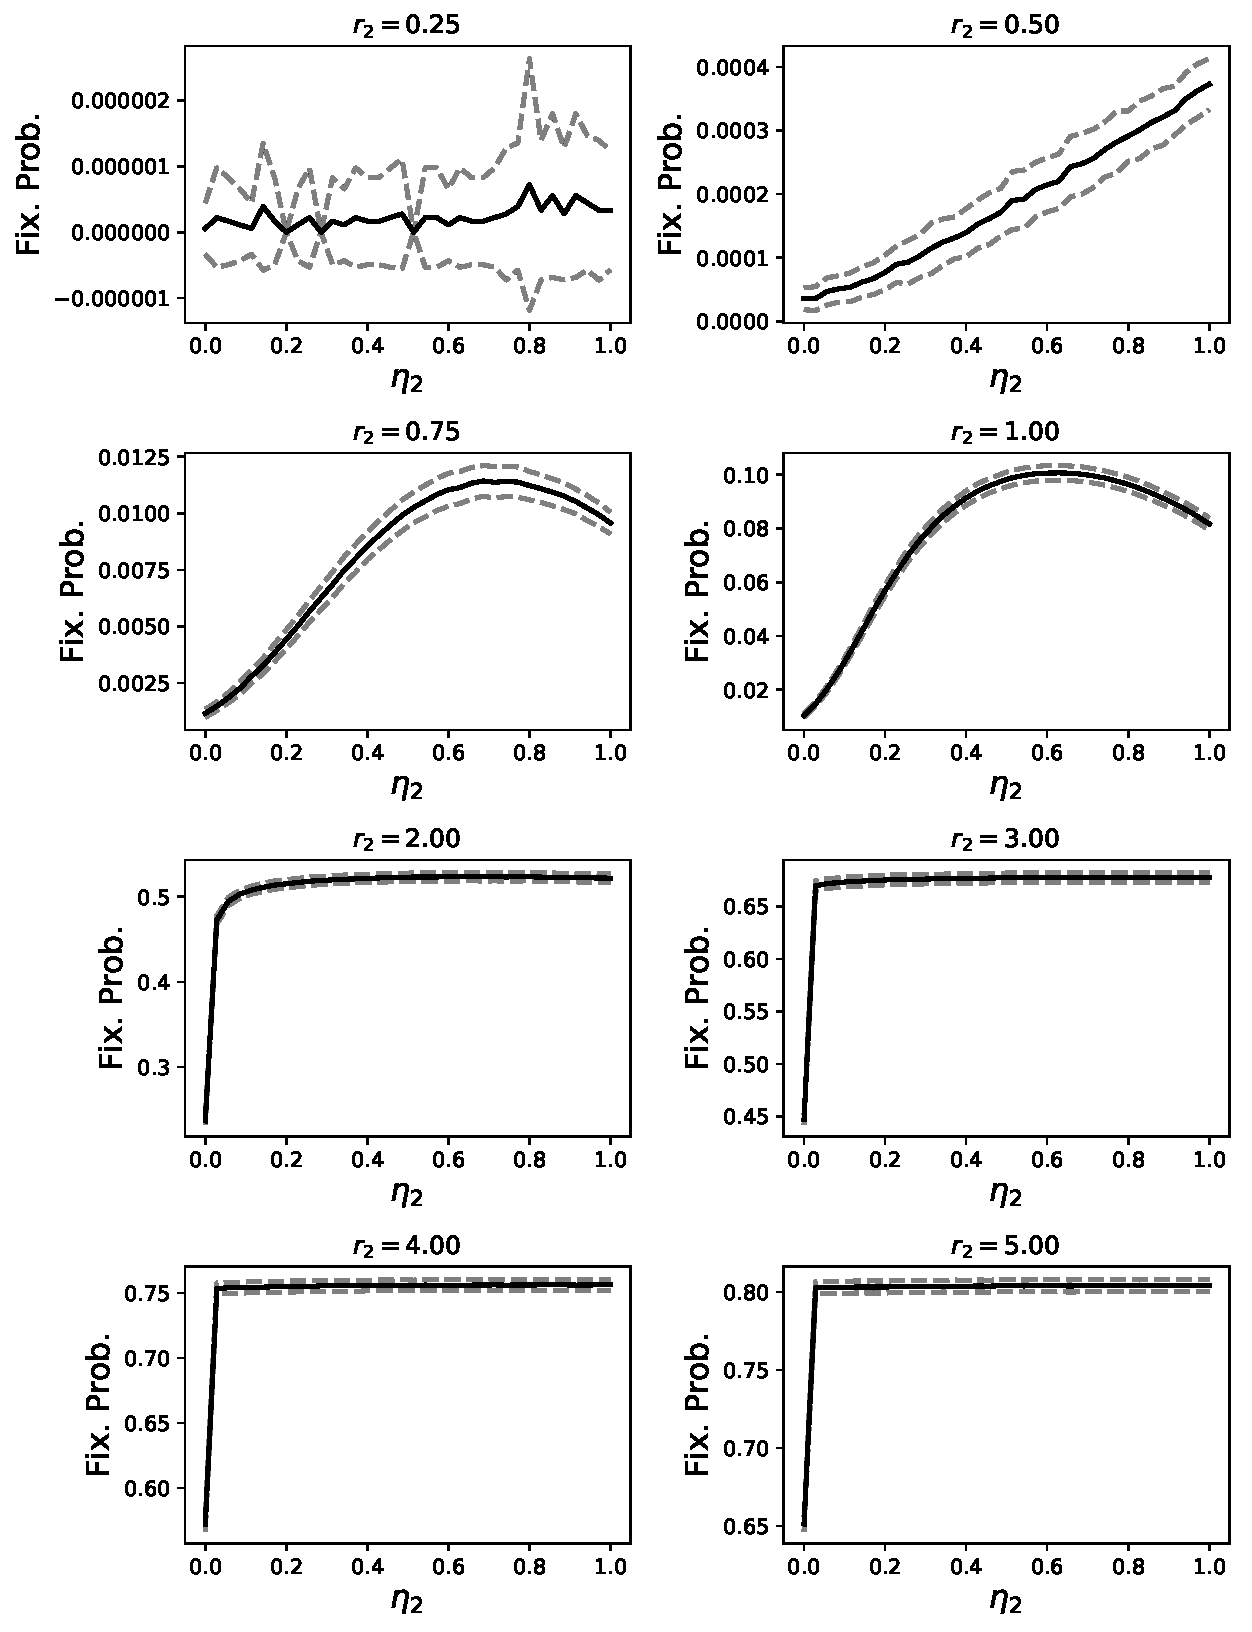
\includegraphics[width=0.74\textwidth]{avg_eta1_r2_stackplot.pdf}
\end{center}
\caption{Average fixation probability for various relative fitness levels of the mutant-type cells, $r_2=\tilde{r}_2$. The dashed lines indicate one deviation of the standard error of the mean. The average was taken over wild-type de-differentiation probability $\eta_1$.}\label{r2_stack}
\end{figure}

The results of Figure \ref{r2_stack} show that for general mutant increasing the relative fitness increases the fixation probability. For cases where the relative fitness is lower, the de-differentiation parameter $\eta_2$ is more important. It is only for relatively larger relative fitness levels that  these fixation probability curves begin to demonstrate saturation and diminishing returns as a response to increased mutant cell plasticity.  In these cases, saturation is reached quicker for larger $r_2=\tilde{r}_2$ values. Thus even small values of $\eta_2$ are sufficient to maximise the chances of fixation. 

However, for relative fitness values that are closer to neutral (i.e. $r_2=\tilde{r}_2=0.75$) we recover the non-monotone behaviour. That is, when there is no substantial advantage between the wild-type and mutant-type stem cells, fixation probability is more complicated than just maximising the plasticity. In these cases, as seen in Section \ref{further}, the behaviour of the stem cells is governed by competing evolutionary pressures and results in a greater need to balance parameters than to maximise parameters.

\begin{figure}[H]
\begin{center}
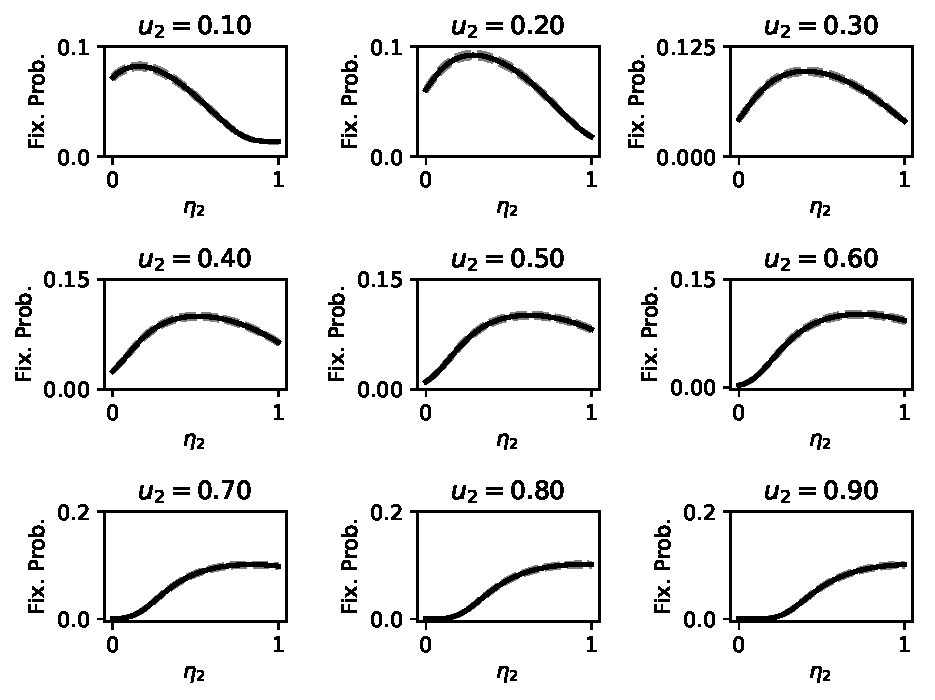
\includegraphics[width=0.74\textwidth]{avg_eta1_u2_stackplot.pdf}
\end{center}
\caption{Average fixation probability for various values of $u_2$, the probability the mutant type stem cell differentiates. The dashed lines indicate one deviation of the standard error of the mean. The average was taken over wild-type de-differentiation probability $\eta_1$.}\label{u2_stack}
\end{figure}

In Figures \ref{u2_stack} the probability parameter $u_2$ was varied. This parameter corresponds to the probability a mutant stem cell will differentiate. These results corroborate the claim that the non-monotonicity of the fixation probability function is a general phenomenon and not a result of careful parameter choice. For smaller $u_2$ values the fixation probability function is more right-skewed and for larger $u_2$ values the function is more left-skewed. In fact, for sufficiently large enough $u_2$ values the resulting function is monotone increasing. 

The left-skew of the small $u_2$ functions indicates that when the mutant cells do not differentiate often, increasing the de-differentiation parameter is worse for fixation. This could be because in order for the wild-type cells to fixate they must selectively eliminate all mutant stem cells and differentiated cells. Hence, if there are few mutant differentiated cells to begin with, removing them from the micro-environment provides a selective advantage to the wild-type cells. When $u_2$ is larger, there are enough differentiated cells in the micro-environment that allowing some to de-differentiate (equivalent to $0<\eta_2<1$) provides a selective advantage for the mutant-type cells. However, allowing too many mutant differentiated cells to de-differentiate (equivalent to $\eta_2\approx 1$) results in the differentiated cell pool depleting too quickly and the resultant selective advantage for the wild-type cells provides a selective disadvantage to the mutant-type cells. For sufficiently large $u_2$ as in the plots for $u_2=0.8$ and $u_2=1$, mutant stem cells are almost always de-differentiating, hence the only way to refill the mutant stem cell pool is to increase the rate of de-differentiation. For these scenarios the bottle-neck for fixation is recovering enough stem cells to create a selective disadvantage on the wild-type cells. Hence, increasing $\eta_2$ is always the most evolutionary effective means of increasing fixation.

\section{Conclusion}
In conclusion, two, apparently contradictory, stochastic models of cancer stem cell behaviour were considered. Both models were questioning the invasive capacity of mutant stem cells in the presence of a pre-existing stem cell and differentiated cell strata. The models were concerned with how the phenotypic plasticity, or de-differentiation rate, affected the invasive potential of these mutant stem cells. A Moran birth-death model was considered and Gillespie simulations of a reaction network were considered. The apparent discrepancy between these models was discovered to be hidden within assumptions determining how both the resident type and mutant type plasticity rates alter. This apparent contradiction was resolved and the behaviour of the Gillespie simulation model was recovered in the Moran context, and vice versa.

It was also observed that increasing plasticity in the mutant type differentiated cells can result in both positive and negative effects for the fixation probability of the mutant stem cells. This seeming contradiction was demonstrated to be stable across differing parameter sets indicating that this phenomenon may be observed in general. 

\section{Acknowledgment}
Financial support by the Natural Sciences and Engineering Research Council of Canada (NSERC)(MK) is gratefully acknowledged. 

\begin{appendices}

\section{Numerics}\label{exp}

The Moran simulations were run until fixation occurred or until 15,000 iterations were achieved -- whichever came first. A total of 500,000 such simulations were run in 50 batches of 10,000. For each batch of 10,000 simulations, fixation probability was estimated by logging what percentage of the 10,000 iterations achieved fixation. The error of these probabilities was estimated as the standard error of the mean calculated between the 50 different batches.  This process was completed once for every unique set of parameter values. 

Similarly, the two Gillespie simulations (in Figures \ref{combine_fig} and \ref{moh_wod_switch}) were run until fixation of or until $10^8$ iterations were achieved. For each parameter set, these simulations were run in 10 batches of 3000 simulations with the fixation probability being calculated for each individual batch of 3000 simulations. The error was calculated from these 10 different fixation probabilities as the standard error of the mean.

\subsection{Figure Information}
In Figure \ref{combine_fig} the leftmost plot was generated by Moran simulations with the following parameters: $N_S=N_D=10$, $u_1=u_2=0.5$, $r_1=r_2=\tilde{r}_1=\tilde{r}_2=1$, $\eta_1=0$, $d_1=d_2=\tilde{d}_1=\tilde{d}_2=1$, and $\eta_2$ varying over 36 discrete values evenly placed between $0$ and $1$, inclusive.

Similarly, the rightmost plot was generated by Gillespie simulations with the following parameters: $r_1'=r_2'=0.5$, $p_1'=p_2'=0.8$, $h_{1,1}=h_{2,1}=h_{1,2}=h_{2,2}=h_{1,3}=h_{2,3}=0.01$, $k_1=k_2=k_3=1$, $\alpha_1=\alpha_2=0.5$
, and $g_1'=g_2'=g$. The initial condition for these simulations was $(S_1, D_1, S_2, D_2) = (S_1^\ast, D_1^\ast, 1, 0)$ where $S_1^\ast$ and $D_1^\ast$ are defined as (within rounding to nearest integer) the equilibrium point of the deterministic differential equations in $S_1$ and $D_1$ (where $S_2$ and $D_2$ are assumed to be zero for the purpose of obtaining the equilibrium values). The stochastic simulation was then repeated for each $g$ value in $\{0, 0.05, 0.1, 0.15, 0.2, 0.25, 0.3\}$. 

%rp, pp, gp, alpha, h1, h2, h3, k1, k2, k3,
%0.5, 0.8, gp, 0.5, 0.01, 0.01, 0.01, 1, 1, 1,

In Figure \ref{moh_wod_switch} the leftmost plot was generated by Moran simulations with the following parameters: $N_S=N_D=10$, $u_1=u_2=0.5$, $r_1=r_2=\tilde{r}_1=\tilde{r}_2=1$, $d_1=d_2=\tilde{d}_1=\tilde{d}_2=1$, and $\eta_1=\eta_2=\eta$ where $\eta$ varies over 36 discrete values evenly placed between $0$ and $1$, inclusive.

Similarly, the rightmost plot was generated by Gillespie simulations with the following parameters:$r_1'=r_2'=0.5$, $p_1'=p_2'=0.8$, $h_{1,1}=h_{2,1}=h_{1,2}=h_{2,2}=h_{1,3}=h_{2,3}=0.01$, $k_1=k_2=k_3=1$, $\alpha_1=\alpha_2=0.5$
, $g_1'=0$, and $g_2'$ taking values in $\{0, 0.05, 0.1, 0.15, 0.2, 0.25, 0.3\}$. As in Figure \ref{combine_fig}, the initial condition was taken to be $(S_1, D_1, S_2, D_2)=(S_1^\ast, D_1^\ast, 1, 0)$ with $S_1^\ast$ and $D_1^\ast$ defined as before.

In Figure \ref{contour} the data was generated with Moran simulations with the following parameters:  $N_S=N_D=10$, $u_1=u_2=0.5$, $r_1=r_2=\tilde{r}_1=\tilde{r}_2=1$, $d_1=d_2=\tilde{d}_1=\tilde{d}_2=1$, and both $\eta_1$ and $\eta_2$ vary, independently, from $0$ to $1$ in $0.1$ increments. A cubic spline was generated from the resulting data points (and their standard errors) and used to create the plots in Figures \ref{constantEta1Stack} and \ref{eta_stack}.

In Figure \ref{avg_eta1_plot} the data was generated, for each fixed $\eta_2$ value, by averaging over all 36 $\eta_1$ values.

Figures \ref{r2_stack} and \ref{u2_stack} were generated similarly. In both figures Moran simulations were run with parameters $N_S=N_D=10$, $d_1=d_2=\tilde{d}_1=\tilde{d}_2=1$, and $\eta_1$ and $\eta_2$ independently varying over 36 discrete values evenly placed between $0$ and $1$, inclusive. In Figure \ref{r2_stack} $r_2=\tilde{r}_2=r$ where $r$ takes on values in $\{0.25, 0.50, 0.75, 1, 2, 3, 4, 5\}$ while $u_1=u_2=0.5$. Similarly, in Figure \ref{u2_stack} $u_2$ was allowed to vary between $0.1$ and $0.9$ inclusive in increments of $0.1$, while $r_2=\tilde{r}_2=1$ and $u_1=0.5$ were kept constant. The averages were calculated from the resulting data points as in Figure \ref{avg_eta1_plot}.

The data, and the code to generate the data, can be found at \url{https://www.github.com/brydon/StemCells2018/}

\end{appendices}

\bibliographystyle{apalike}
\bibliography{project}
\end{document}
